\documentclass[12pt,a4paper]{article}

\usepackage{epcc}
\usepackage{graphicx}
\usepackage{listings}
\usepackage{color}
\usepackage{amsmath}

\definecolor{mygreen}{rgb}{0,0.6,0}
\definecolor{mygray}{rgb}{0.5,0.5,0.5}
\definecolor{mymauve}{rgb}{0.58,0,0.82}

\lstset{ 
	backgroundcolor=\color{white},   % choose the background color; you must add \usepackage{color} or \usepackage{xcolor}; should come as last argument
	basicstyle=\footnotesize,        % the size of the fonts that are used for the code
	breakatwhitespace=false,         % sets if automatic breaks should only happen at whitespace
	breaklines=true,                 % sets automatic line breaking
	captionpos=b,                    % sets the caption-position to bottom
	commentstyle=\color{mygreen},    % comment style
	deletekeywords={...},            % if you want to delete keywords from the given language
	escapeinside={\%*}{*)},          % if you want to add LaTeX within your code
	extendedchars=true,              % lets you use non-ASCII characters; for 8-bits encodings only, does not work with UTF-8
	frame=single,	                   % adds a frame around the code
	keepspaces=true,                 % keeps spaces in text, useful for keeping indentation of code (possibly needs columns=flexible)
	keywordstyle=\color{blue},       % keyword style
	language=C,                 	 % the language of the code
	morekeywords={*,...},            % if you want to add more keywords to the set
	numbers=left,                    % where to put the line-numbers; possible values are (none, left, right)
	numbersep=5pt,                   % how far the line-numbers are from the code
	numberstyle=\tiny\color{mygray}, % the style that is used for the line-numbers
	rulecolor=\color{black},         % if not set, the frame-color may be changed on line-breaks within not-black text (e.g. comments (green here))
	showspaces=false,                % show spaces everywhere adding particular underscores; it overrides 'showstringspaces'
	showstringspaces=false,          % underline spaces within strings only
	showtabs=false,                  % show tabs within strings adding particular underscores
	stepnumber=5,                    % the step between two line-numbers. If it's 1, each line will be numbered
	stringstyle=\color{mymauve},     % string literal style
	tabsize=2,	                     % sets default tabsize to 2 spaces
	title=\lstname                   % show the filename of files included with \lstinputlisting; also try caption instead of title
}

\usepackage{hyperref}
\hypersetup{
	colorlinks=true, %set true if you want colored links
	linkcolor=black,  %choose some color if you want links to stand out
}

\newcommand{\sectionVspacing}{\vspace{15pt}} 


\begin{document}

\title{Threaded Programming Coursework Part 2}
\author{Exam number B136013}
\date{\today}

\makeEPCCtitle

\thispagestyle{empty}

\newpage
\clearpage

\tableofcontents

\newpage
\clearpage

\section{Introduction}

The goal of this coursework is to implement an alternative loop scheduling algorithm using OpenMP API. The scheduling method is called Affinity scheduling and it will be described in the following section.

\sectionVspacing

\section{Project Specification}
\subsection{Description}

In short, Affinity scheduling assigns a local set of iterations of the given loop to each thread. When each thread finishes these iterations it will search into the other threads, it will find the most loaded one and it will take a fraction of its workload.

\subsection{Terminology}

In order to analyze the design, the definition of basic terminology is required. These terms are explained in this section.

\begin{itemize}
  \item Chunk: A contiguous, non-empty subset of the iterations of a loop.
  \item Chunksize: The number of iterations for a specific Chunk.
  \item Local Set: A contiguous set of iterations assigned to each thread. In this case, the size of an initial Local Set is n/p, where n is the number of iterations for the running loop and p the number of threads.
  \item Most Loaded thread: At a specific time, the thread with the most remaining iterations of its given Local Set.
\end{itemize}

\sectionVspacing

\section{Analysis}

\subsection{Tools}

The programming language used for the development of the scheduler is C. As regards the compiler we have used GCC from the GNU Compiler Collection including the -O3 option to ensure a high level of optimization in the sequential part of the problem. In terms of building, GNU Make rules made to compile, run and clean the project.

\subsection{Design}

The scheduler's design is pretty straightforward containing the necessary data structures and functions that hold vital information about the progress of the loop and each thread workload. The functions containing the body of the loop has not been changed. The only modifications made are in runloop function providing the right Chunks for the loop.

First and foremost, we created an initialization function that only one of the threads has to execute (first come, first served). This function takes as input the number of iterations in the loop and the number of the active threads for this job. To be more specific, this method creates a structure that contains an array of Local Sets. The index in this array is the number of the current thread. 

For example, if we want to obtain the Local Set for thread number 4, the only thing we have to do is to look up for the fourth structure in the array.
A Local Set in our implementation is a data structure containing the starting position for the next to execute chunk, the highest iteration to be calculated for this Local Set and last but not least an omp\_lock\_t that a thread is forced to obtain in order to update the Local Set.

The main interest lies in the function that returns the next Chunk (more in Synchronization section). The next Chunk is just a structure containing the lowest and highest position that the thread has to run in the loop.

It worths mentioning that each time a thread finishes the execution for the given Chunk checks if the loop has finished. A loop has finished if each Local Set's lowest position equals the highest one. If this is not true then it tries again to take the next Chunk (if it is possible).

At the end of the loop, a function is called that is responsible to free the allocated head memory for the Local Sets. Just like the initialization phase, this method is called by the thread that arrives first in this section.

\subsection{Syncronization}

As mentioned before, synchronization is needed in the system to obtain the next Chunk. In terms of correctness, the implementation of this function has to ensure that each iteration is going to run exactly one time by one thread. Also, for efficiency reasons race conditions between threads have to be reduced in a specific manner to avoid deadlocks.

The process is very simple. In the beginning, the thread tries to acquire the next Chunk from its Local Set if this is successful it returns with the Chunk if not it has to steal workload for the most loaded thread.

To find the most loaded thread we have to iterate the array of the Local Sets, peek the remaining workload and if it is the biggest seen until now we try to lock it and acquire it as the next to execute Chunk. If the Chunksize is smaller than the one that we have found in this array we ignore it without any attempt to lock it. We can denote that this approach speeds up the process without unnecessary locks for less loaded Chunks. 

Our most loaded Local Set remains locked to avoid any other threads trying to steal it from us. When the scan is completed and it is assured that the most loaded Local Set is taken, we update the indexes and then unlock it. The update means that the lowest index is increased by the size of the new Chunksize. The new Chunksize is simply the remaining load of the Local Set divided by the number of threads. In this way, we guarantee that the selected Chunk is not executed by another thread. 

Waiting to obtain the lock for the next Local Set is unavoidable, but deadlocks are eliminated because no matter what happens each thread will eventually unlock the selected Local Set.

\sectionVspacing

\section{Evaluation}

We have evaluated the scheduler running our experiments on the backend of Cirrus supercomputer using 1, 2, 4, 6, 8, 12 and 16 threads. Then, we compared our results with the best scheduling options that we found in coursework 1 (guided, 4 for Loop 1 and dynamic, 16 for Loop 2). The evaluation process includes graphs for each loop of the running time and the speedup against the number of threads. In addition, the speedup graphs contain the ideal measurements based on Amdahl's law.

It worths mentioning that the measurements are a product of multiple runs over the loops. To be more specific each of the loops has been executed 20 times. Then the mean values have been used for the visual representations.

\subsection{Loop 1}

\subsubsection{Running Time}

There is no denying the fact that running time for loop 1 is identical for guided, 4 and affinity scheduling options based on Figure 1. This happens because for the specific problem the schedulers operate more or less the same way.

Each of them takes an initial local set to run, based on the remaining load size and number of threads. Then dynamically finds the next fraction to execute. The size of this fraction is again calculated by the workload and number threads in both scheduling options.

The only difference worth pointing out, in this case, is when the number of threads is small. Let's take the case running with two threads. In Guided, 4 scheduling the first thread is obliged to execute the first half of the heaviest weight iterations. In contrast, in affinity scheduling, the first Local Set will be possibly executed by both of the threads. This happens because the second Local Set contains fewer calculations. Eventually, if we add the race conditions over the first Local Set we end up with one thread delaying the other. This communication overhead results to the same execution time for both of the scheduling options.

As we increase the number of threads, on both occasions Chunksizes become smaller. We have not a single thread carrying all of the work so communication is the only drawback. All of the threads in both of the scheduling options race in taking the next Chunk. This behavior again concludes to the same running time between our cases.

\begin{figure}[ht]
    \centering
    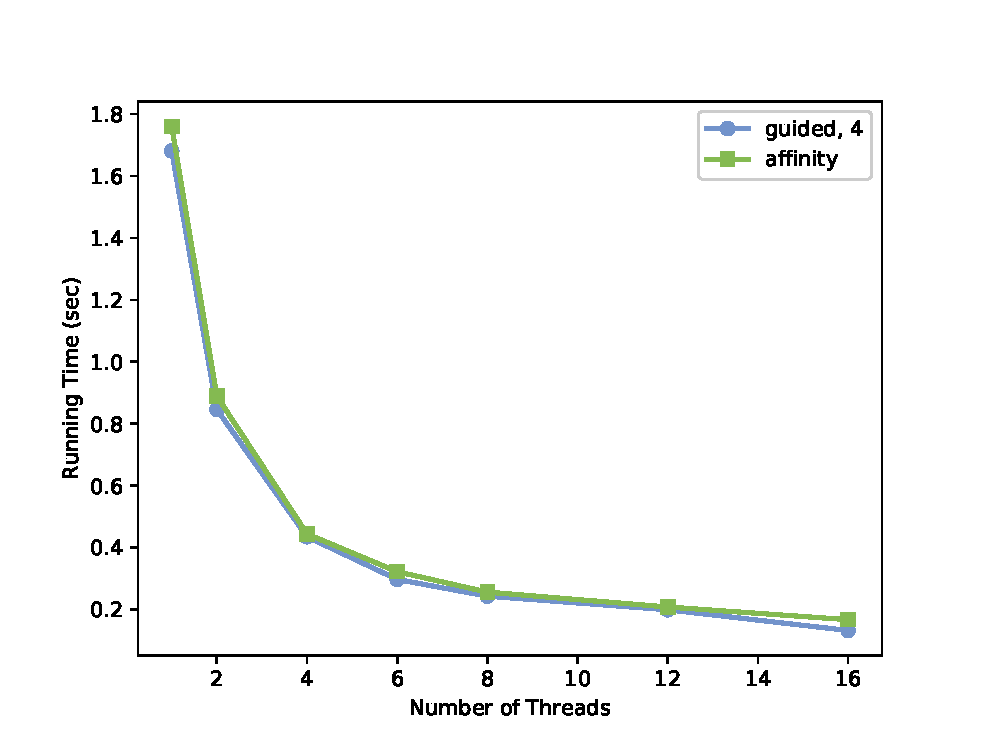
\includegraphics[scale=0.6]{../graphs/loop1_running_time.eps}
    \caption{Running Time Loop 1}
    \label{Running Time Loop 1}
\end{figure}

\subsubsection{Speedup}

When it comes to scalability affinity scheduling speeds up in a nearly linear fashion for 1 to 8 threads based on Figure 2. As long as we increase the number of threads beyond that point the rate of change declines slightly.

The basic difference between the ideal and affinity speedup in the communication overhead when more and more threads are used the Chunksize is becoming even smaller and the need to obtain the next Chunk bigger. This characteristic leads to more race conditions. As a result, the delay is unavoidable so we could say that using 6 or 8 threads would be the optimal approach to solve this problem.

\begin{figure}[ht]
    \centering
    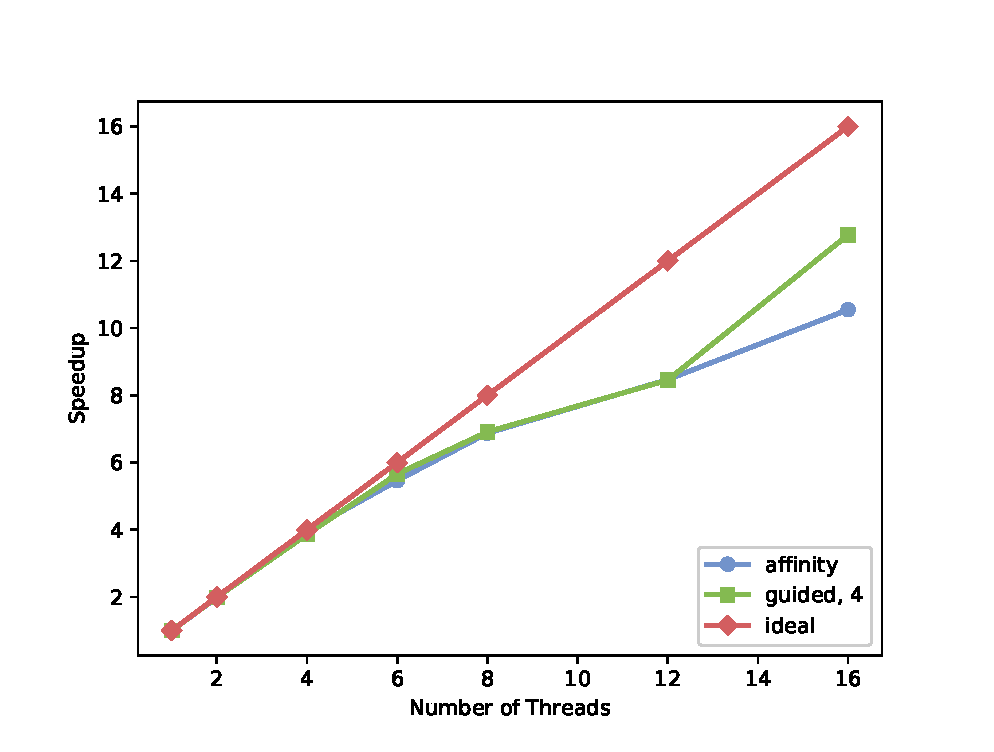
\includegraphics[scale=0.6]{../graphs/loop1_speedup.eps}
    \caption{Speedup Loop 1}
    \label{Speedup Loop 1}
\end{figure}

\subsection{Loop 2}

\subsubsection{Running Time}

When it comes to Loop 2 there are some interesting observations. Running with 1 to 6 threads based on Figure 3 the dynamic, 16 option seems much faster and scalable than affinity. Then the trend changes, dynamic scheduling preserves a constant running time but the affinity keeps improving.

To be more specific, running the loop with 1 to 6 threads dynamic, 16 is the best configuration for this problem. This happens because, for the first outer iterations which are the most loaded, the threads share equally the calculations without the communication been an overhead. As we increase the number of threads those who take the latest Chunks are underutilized and consume most of the time in obtaining the next lightweight Chunk.

In contrast, the affinity scheduling option is more scalable for the whole experiment but with tinier changes in running time. As we increase the threads number when the latest of them finish with their Local Set, more are available to contribute calculation the first heavyweight iterations.

To sum up, the basic difference between these two scheduling options is that the affinity is able to redistribute heavy workload to other threads with a variety of Chunksize but dynamic is bound to calculate 16 iterations each time which is not optional for each of the threads configurations.

\begin{figure}[ht]
    \centering
    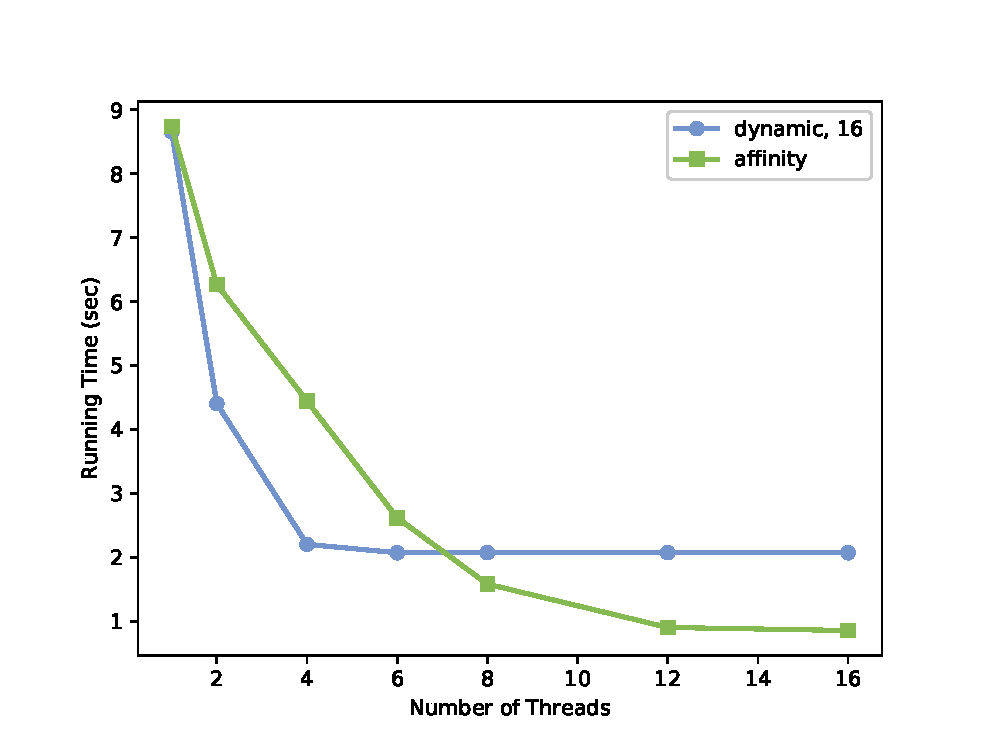
\includegraphics[scale=0.6]{../graphs/loop2_running_time.eps}
    \caption{Running Time Loop 2}
    \label{Running Time Loop 2}
\end{figure}

\subsubsection{Speedup}

When we compare the speedup of affinity scheduling with the ideal, as we increase the number of threads, Chunksizes become smaller so the workload is easier to be distributed. That happens until we use 6 threads, after that point again the communication becomes an overhead the speedup begins to decline like in Loop 1.

\begin{figure}[ht]
    \centering
    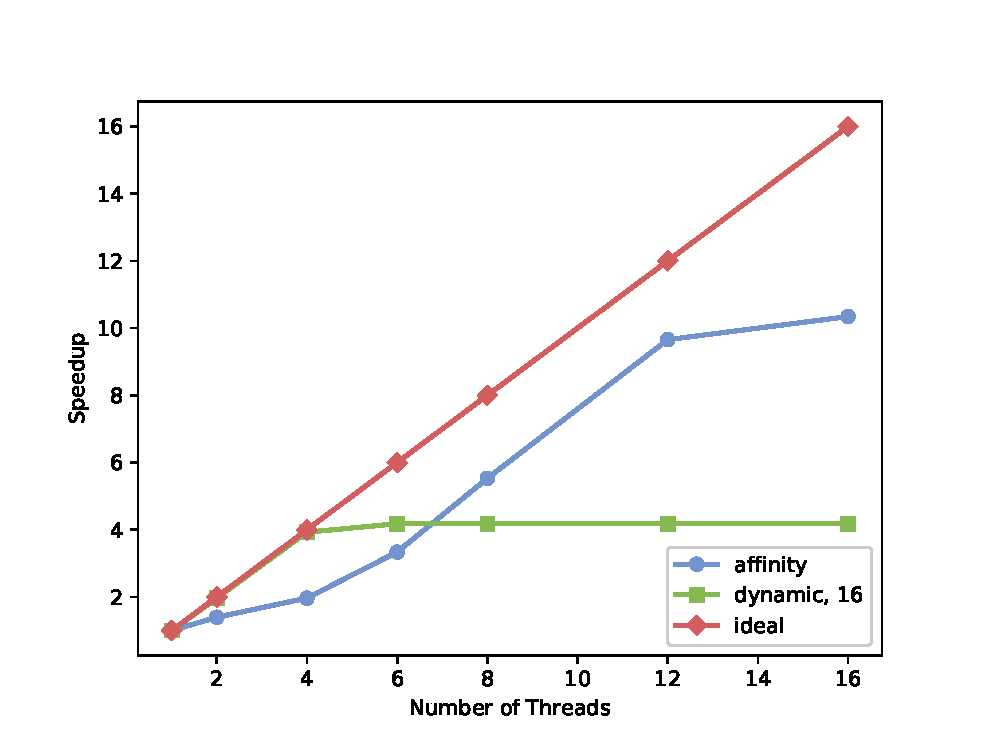
\includegraphics[scale=0.6]{../graphs/loop2_speedup.eps}
    \caption{Speedup Loop 2}
    \label{Speedup Loop 2}
\end{figure}

\sectionVspacing

\section{Conclusion}
In conclusion, the affinity scheduling option is optimal for loops that the workload is equally distributed in different iterations. If this not the case, lightweight threads can steal workload from the heavyweight Local Sets which is a good load balancing approach. As we approach the end of the loop this happens to be the bottleneck because the Chunks become smaller. Giving an option to the scheduler for the smallest Chunksize could solve this problem reducing redundant race conditions between the threads.

\end{document}
